\documentclass[11pt]{article}


\usepackage{fullpage}
\usepackage{graphicx}
\usepackage{amsmath}
\usepackage{amssymb}
\usepackage{amsthm}
\usepackage{fancyvrb}

\newcommand{\myname}{Mehshan Mustafa}

\newenvironment{theorem}[2][Theorem]{\begin{trivlist}
\item[\hskip \labelsep {\bfseries #1}\hskip \labelsep {\bfseries #2.}]}{\end{trivlist}}
\newenvironment{lemma}[2][Lemma]{\begin{trivlist}
\item[\hskip \labelsep {\bfseries #1}\hskip \labelsep {\bfseries #2.}]}{\end{trivlist}}
\newenvironment{exercise}[2][Exercise]{\begin{trivlist}
\item[\hskip \labelsep {\bfseries #1}\hskip \labelsep {\bfseries #2.}]}{\end{trivlist}}
\newenvironment{problem}[2][Problem]{\begin{trivlist}
\item[\hskip \labelsep {\bfseries #1}\hskip \labelsep {\bfseries #2.}]}{\end{trivlist}}
\newenvironment{question}[2][Question]{\begin{trivlist}
\item[\hskip \labelsep {\bfseries #1}\hskip \labelsep {\bfseries #2.}]}{\end{trivlist}}
\newenvironment{corollary}[2][Corollary]{\begin{trivlist}
\item[\hskip \labelsep {\bfseries #1}\hskip \labelsep {\bfseries #2.}]}{\end{trivlist}}
\newenvironment{solution}{\begin{proof}[Solution]}{\end{proof}}
\newenvironment{idea}[2][Proof Idea.]{\textit{#1} #2}



\parindent0in
\pagestyle{plain}
\thispagestyle{plain}

\usepackage{csquotes}
\usepackage[shortlabels]{enumitem}

\newcommand{\dated}{\today}
\newcommand{\token}[1]{\langle \text{#1} \rangle}

\begin{document}

\textbf{Introduction to the Theory of
Computation}\hfill\textbf{\myname}\\[0.01in]
\textbf{Chapter 7: Time Complexity}\hfill\textbf{\dated}\\
\smallskip\hrule\bigskip

\begin{problem}{7.27}
A cut in an undirected graph is a separation of the vertices $V$ into two disjoint
subsets $S$ and $T$. The size of a cut is the number of edges that have one endpoint
in $S$ and the other in $T$. Let
\[
MAX\text{-}CUT = \{\langle G, k \rangle \ | \ G \text{ has a cut of size } k \text{ or more}\}.
\]
Show that $MAX\text{-}CUT$ is NP-complete. You may assume the result of Problem 7.26.
\end{problem}

\begin{proof}
To show that $MAX\text{-}CUT$ is NP-complete, we must show that it is in NP and that all NP-problems are polynomial time reducible to it. The first part is easy; a certificate is simply two disjoint subsets of $V$ having cut size of $k$ or more. To prove the second part, we show that $\neq$\textit{SAT} is polynomial time reducible to $MAX\text{-}CUT$. \\

The reduction converts a 3cnf-formula $\phi$ into an undirected graph $G$ and
a number $k$, so that $\phi$ has a satisfying $\neq$\textit{-assignment}, iff G has a cut of size $k$ or more. The graph contains gadgets that mimic the variables and clauses of the formula. \\

The variable gadget for variable $x$ is a collection of $3c$ nodes labeled with $x$ and another $3c$ node labeled with $\overline{x}$, where $c$ is the number of clauses. All nodes labeled $x$ are connected with all nodes labeled $\overline{x}$. The clause gadget is a triangle of three edges connecting three nodes labeled with the literals appearing in the clause. Do not use the same node in more than one clause gadget. Finally, we choose $k$ to be the maximum possible cut size of $l \times (3c)^2 + 2c$ in $G$, where $l$ is the number of variables in $\phi$. \\

Suppose that $\phi$ has satisfying $\neq$\textit{-assignment}. Such an assignment to the variables of $\phi$ is one where each clause contains two literals with unequal truth values. In graph $G$, the vertices $V$ can be paritioned into two disjoint subsets $S$ and $T$ as follows:
\begin{enumerate}
\item If some variable $x$ is assigned true value, then put $x$ nodes in $S$ and $\overline{x}$ nodes in $T$.
\item If some variable $x$ is assigned false value, then put $x$ nodes in $T$ and $\overline{x}$ nodes in $S$.
\end{enumerate}

Clearly, in this parition all the $l \times (3c)^2$ edges in variable gadgets have one endpoint in $S$ and other in $T$. Next, we show that the clause gadgets have $2c$ edges that have one endpoint in $S$ and other in $T$. Let $c_i$ be any clause $(y_1 \vee y_2 \vee y_3)$ in $\phi$. Every clause $c_i$ contains two literals with unequal truth values. These two literals can be:
\begin{enumerate}
\item Same variable $x$ and $\overline{x}$.
\item Different variables, where both literals are non-negated $x$ and $y$.
\item Different variables, where one literal is negated $\overline{x}$ and $y$.
\item Different variables, where both literals are negated $\overline{x}$ and $\overline{y}$.
\end{enumerate}

In each case, a clause gadget has two edges that have one endpoint in $S$ and other in $T$. Therefore, the graph $G$ has a cut size of $l \times (3c)^2 + 2c$ or more. \\

Suppose the graph $G$ has a cut size of $l \times (3c)^2 + 2c$ or more. Then, the separation of the vertices $V$ into two disjoint subsets $S$ and $T$ gives the $\neq$\textit{-assignment} for $\phi$. If a node $x_i$ is in $S$, then the variable $x_i$ is assigned true, otherwise false.

\end{proof}

\begin{center}
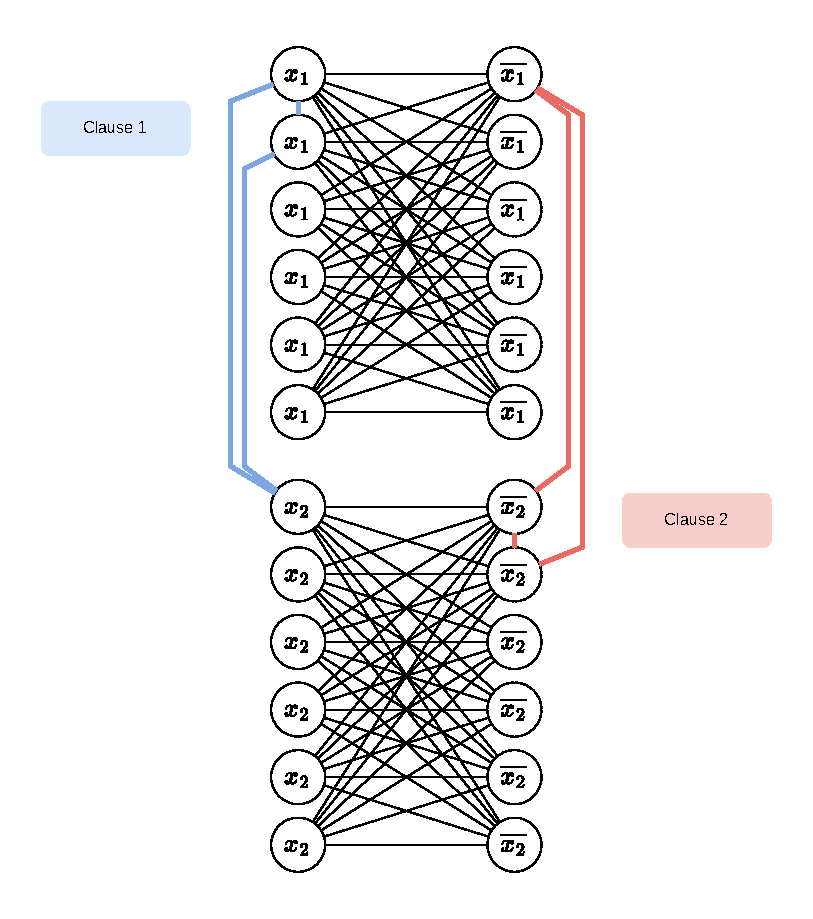
\includegraphics[scale=1.0]{Figures/Problem7.27a.pdf} \\
Graph $G$ for $\phi = (x_1 \vee x_1 \vee x_2) \wedge (\overline{x_1} \vee \overline{x_2} \vee \overline{x_2})$. \\ Maximum cut size is obtained  when $S$ contains \\ all nodes labeled $x_1$ and $\overline{x_2}$, and $T$ contains nodes \\ $\overline{x_1}$ and $x_2$.
\end{center}

\end{document}